\pagebreak
\thispagestyle{empty}
\movetoevenpage
\begin{figure}
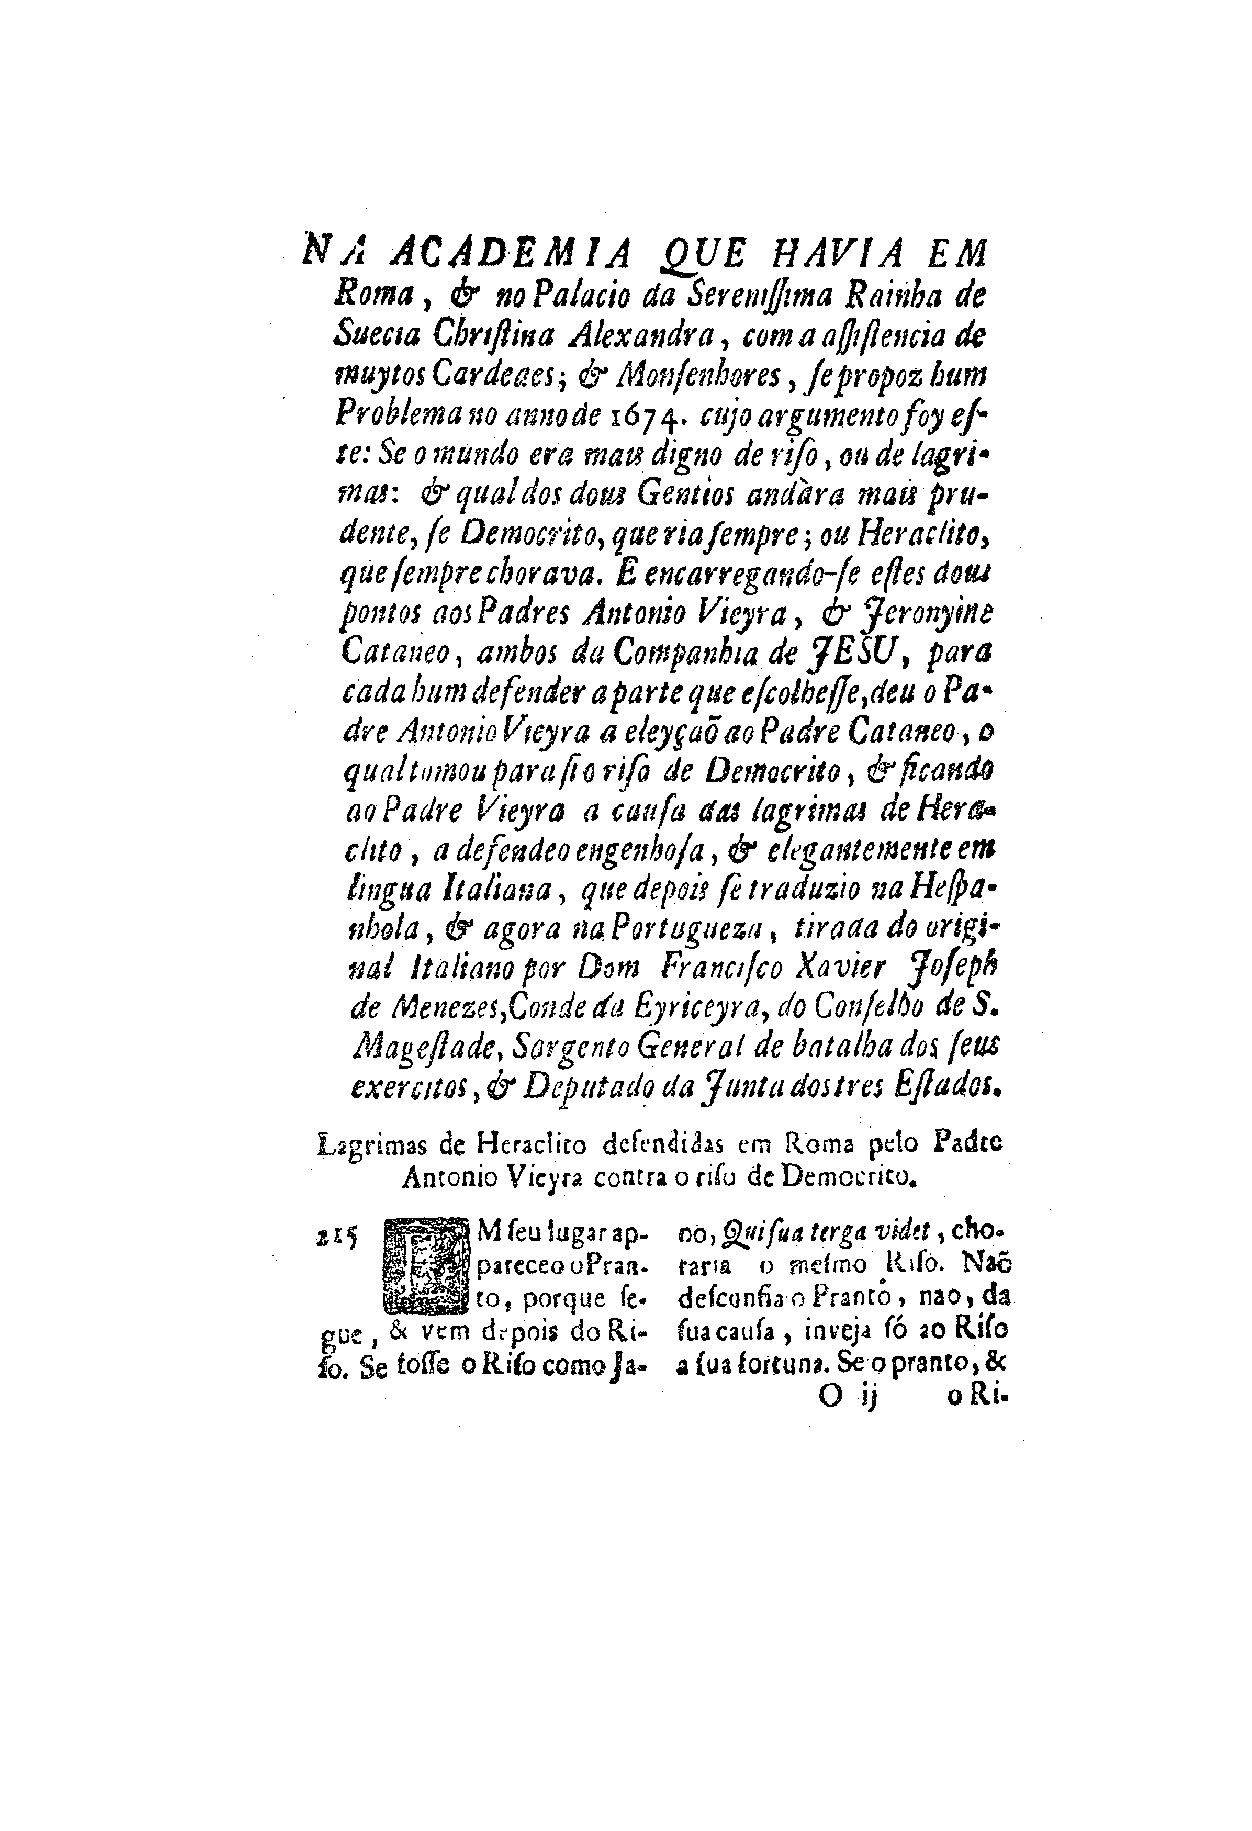
\includegraphics[width=\textwidth]{./imgs/heraclito.pdf}  
\end{figure}

\chapter{Lágrimas de Heráclito}


\begin{quotation}
\noindent{}Na academia que havia em Roma, 65° no Palácio da Sereníssima Rainha de
Suécia Cristina Alexandra, com a assistência de muitos Cardeais, e
Monsenhores, se propôs um Problema no ano de 1674, cujo argumento foi
este: Se o mundo era mais digno de riso, ou de lágrimas: e qual dos dois
gentios andara mais prudente, se Demócrito, que ria sempre; ou
Heráclito, que sempre chorava. E encarregando"-se estes dois pontos aos
Padres Antônio Vieira, e Jerônimo Cataneo, ambos da Companhia de Jesus
para cada um defender a parte que escolhesse, deu o Padre Antônio Vieira
a eleição ao Padre Cataneo, o qual tomou para si o riso de Demócrito, e
ficando ao Padre Vieira a causa das lágrimas de Heráclito, a defendendo
engenhosa e elegantemente em língua italiana, que depois se traduziu na
Espanhola e agora na Portuguesa, tirada do original italiano por Dom
Francisco Xavier José de Menezes, Conde da Eiriceira, do Conselho de S.\,Majestade, Sargento General de batalha dos seus exércitos, e Deputado da
Junta dos Três Estados.
\end{quotation}

\noindent{}Em seu lugar apareceu o pranto, porque segue e vem depois do riso. Se
fosse o riso como Jano, \emph{qui sua terga videt}, choraria o mesmo riso. Não
desconfia o pranto,
não, da sua causa: inveja só ao riso a sua fortuna. Se o pranto e o riso
aparecessem neste grande teatro no traje da verdade (sempre nua), sem
dúvida seria a vitória do pranto. Mas vestido, ornado e armado de uma
tão superior eloquência, que o riso se ria do pranto, não é merecimento,
foi sorte. De tudo quanto ri saiu vestido, ornado, e armado o riso: riem
os prados, e saiu vestido de flores; ri"-se a aurora, e saiu ornado de
luzes; e se aos relâmpagos e raios chamou a antiguidade \emph{risus
Vestae et Vulcani}, entre tantos relâmpagos, trovões e raios de
eloquência, quem não julgará ao miserável pranto cego, atônito, e
fulminado? Tal é a fortuna ou a natureza destes dois contrários. Por
isso nasce o riso na boca, como eloquente, e o pranto nos olhos, como
mudo. Mas se \emph{interdum lacrimae pondera vocis habent}, assim mudo,
e com lágrimas, assim triste, e vestido de luto (como costumavam os réus no
Senado da antiga Roma) se apresenta hoje o pranto diante da majestade
do sólio real e tribunal retíssimo dos seus eminentíssimos juízes, não
presumindo que há de alcançar vitória ou aplauso, mas esperando a
piedade e comiseração, que nunca negaram aos miseráveis e aflitos, os
espíritos generosos e magnânimos.

Entrando, pois, na questão, se o mundo é mais digno de riso ou de
pranto, e se à vista do mesmo mundo tem mais razão quem ri, como ria
Demócrito, ou quem chora, como chorava Heráclito, eu, para defender,
como sou obrigado, a parte do pranto, confessarei uma coisa e direi
outra. Confesso que a primeira propriedade do racional é o risível, e
digo que a maior impropriedade da razão é o riso. O riso é o sinal do
racional, o pranto é o uso da razão. Para confirmação desta, que julgo
evidência, não quero mais prova que o mesmo mundo, nem menor prova que o
mundo todo. Quem conhece verdadeiramente o mundo, precisamente há de
chorar, e quem ri, ou não chora, não o conhece.

Que é este mundo, senão um mapa universal de misérias, de trabalhos, de
perigos, de desgraças, de mortes? E à vista de um teatro imenso, tão
trágico, tão funesto, tão lamentável, aonde cada reino, cada cidade e
cada casa continuamente mudam a cena, aonde cada sol que nasce é um
cometa, cada dia que passa um estrago, cada hora e cada instante mil
infortúnios, que homem haverá (se acaso é homem) que não chore? Se não
chora, mostra que não é racional; e se ri, mostra que também são
risíveis as feras.

Mas, se Demócrito era um homem tão grande entre os homens, e um filósofo
tão sábio, e se não só via este mundo, mas tantos mundos, como ria?
Poderá dizer"-se que ele ria, não deste nosso mundo, mas daqueles seus
mundos.

E com razão, porque a matéria de que eram compostos os seus mundos
imaginados, toda era de riso. É certo, porém, que ele ria neste mundo, e
que se ria deste mundo. Como, pois, se ria ou podia rir"-se Demócrito do
mesmo mundo e das mesmas coisas que via e chorava Heráclito? A mim,
senhores, me parece que Demócrito não ria, mas que Demócrito e Heráclito
ambos choravam, cada um a seu modo.

Que Demócrito não risse eu o provo: Demócrito ria sempre; logo nunca
ria. A consequência parece difícil, e é evidente. O riso, como dizem
todos os filósofos, nasce da novidade e da admiração, e cessando a
novidade, ou a admiração, cessa também o riso; e como Demócrito se ria
dos ordinários desconcertos do mundo, e o que é ordinário, e se vê
sempre, não pode causar admiração nem novidade, segue"-se que nunca ria
rindo sempre, pois não havia matéria que lhe motivasse o riso.

Nem se pode dizer que Demócrito se incitava a rir de alguma coisa que
visse ou encontrasse de novo, porque sempre e em todo o lugar ria, e
quando saía de casa já saía rindo: logo, ria do que já sabia; logo, ria
sem novidade nem admiração; logo, o que nele parecia riso não era riso.

Confirma"-se mais esta verdade com o motivo e intenção de Demócrito,
porque não pode haver riso que se não origine de causa que agrade: tudo
o de que Demócrito se ria, não só lhe desagradava muito, mas queria
mostrar que lhe desagradava; logo, não se ria; e se não ria, que era o
que fazia, a que todos chamavam riso? Já disse que era pranto, e que
Demócrito chorava, mas por outro modo. Ora, vede.

Há chorar com lágrimas, chorar sem lágrimas e chorar com riso: chorar
com lágrimas é sinal de dor moderada; chorar sem lágrimas é sinal de
maior dor; e chorar com riso é sinal de dor suma e excessiva. Para prova
da primeira e segunda diferença de chorar com lágrimas, ou sem elas, é
notável o exemplo que refere Heródoto de Psaminito, rei do Egito.

Perdendo Psaminito o reino, viu em primeiro lugar suas filhas vestidas
como escravas, e não chorou; viu depois seu filho primogênito descalço e
carregado de ferros, com mãos atadas e um freio na boca, e não chorou; e
vendo este mesmo Psaminito, e com o mesmo coração, que um seu antigo
criado pedia esmola, derramou infinitas lágrimas. Oh! grande rei e
grande intérprete da natureza! Chora com lágrimas a miséria do criado, e
sem lágrimas a desgraça dos filhos; assim respondeu ele à
pergunta de Cambises: \emph{Domestica mala graviora sunt quam ut
lacrymas recipiant}.
Com o mesmo pensamento, não menos régio nem menos varonil, Hécuba, com
a coroa perdida e a pátria abrasada, proibiu as lágrimas às damas de
Troia, dizendo"-lhes assim:

\begin{verse}
\emph{Quid effuso genas fletu rigatis?}\\
\emph{Levia perpessae sumus, si flenda patimu}\footnote{Senec. in Trag.}
\end{verse}

A dor moderada solta as lágrimas, a grande as enxuga, as congela e as
seca. Dor que pode sair pelos olhos não é grande dor; por isso não
chorava Demócrito, e, como era pequena demonstração da sua dor, não só
chorar com lágrimas, mas ainda sem elas, para declarar"-se com o sinal
maior, sempre se ria.

Nada digo que seja contrário aos princípios da
verdadeira filosofiae da experiência. A mesma causa, quando é moderada e
quando é excessiva produz efeitos contrários: a luz moderada faz ver, a
excessiva cegar; a dor que não é excessiva rompe em vozes, a excessiva
emudece. Desta sorte, a tristeza, se é moderada, faz chorar, se é
excessiva, pode fazer rir; no seu contrário temos o exemplo: a alegria
excessiva faz chorar, e não só destila as lágrimas dos corações
delicados e brandos, mas ainda dos fortes e duros. Quando Minúcio, livre
do cativeiro, apareceu ao seu exército, que era o romano: \emph{In
laetitiam tota castra effusa sunt, ut prae gaudio militibus omnibus lacrimae
manarent},\footnote{Plutarch. in Fab.} diz Plutarco. Pois, se a excessiva alegria é causa do pranto, a excessiva
tristeza, por que não será causa do riso? A ironia tem contrária
significação do que soa: o riso de Demócrito era ironia do pranto: ria,
mas ironicamente, porque o seu riso era nascido de tristeza, e também a
significava; eram lágrimas transformadas em riso por metamorfoses da
dor; era riso, mas com lágrimas, como aquele de quem disse Estácio:

\begin{verse}
\emph{Lacrymosos impia risus audiit}.
\end{verse}

Na guerra morrem muitos soldados rindo, e a razão é, diz Aristóteles
porque são feridos no diafragma: não ria Demócrito como contente: ria
como ferido; recebia dentro do peito todos os golpes do mundo, e tão mal
ferido ria.

Os olhos com injustiça se puderam queixar desta minha filosofia: o
pranto chamava"-se assim porque se batiam as mãos uma com a outra quando
se chorava, porque para chorar não são precisos os olhos, e não seria
próvida a natureza se, havendo sido a origem de tantos pesares, lhes
desse um só desafogo; e, se choram as mãos, a boca, por que não há de
chorar? Heráclito chorava com os olhos, Demócrito chorava com a boca; o
pranto dos olhos é mais fino, o da boca é mais mordaz, e este era o
pranto de Demócrito. De sorte que, na minha consideração, não só
Héráclito, mas Demócrito chorava, só com a diferença de que o pranto de
Heráclito era mais natural, o pranto de Demócrito mais esquisito, e tudo
merece este mundo, digno de novos e esquisitos prantos, para ser
bastantemente chorado.

Mas porque esta minha suposição me separa do problema, e pode parecer
que, como muitas vezes sucede, me aparte da opinião comum para fugir da
dificuldade, seja embora o riso de Demócrito verdadeiro e próprio riso,
apareçam em juízo um e outro filósofo, para que, ouvidos ambos, se veja
claramente a razão de cada um, e confio do merecimento da causa, que
será tão justa a sentença, que Demócrito saia chorando, e Heráclito
rindo.

Sêneca, no livro \emph{De Tranquillitate}, falando destes dois filósofos, dá a
razão por que sempre ria um, e chorava outro, com estas judiciosas
palavras: \emph{Hic, quoties in pubblicum processerat, flebat, ille
ridebat: huic omnia,quae agimus, miseriae, illi ineptiae videbantur}:
Demócrito ria, porque todas as coisas humanas lhe pareciam ignorâncias;
Heráclito chorava, porque todas lhe pareciam misérias: logo, maior razão
tinha Heráclito de chorar que Demócrito de rir, porque neste mundo há
muitas misérias que não são ignorâncias, e não há ignorância que não
seja miséria.

As misérias e os trabalhos que padecem os mortais, ou por obrigação da
natureza, ou por remédio da fortuna, ou por sustento da vida, ou por
conservação do estado particular e público, são misérias, mas não são
ignorâncias, porque as governa a prudência, por necessidade, por
conveniência, por honra e por decoro.

Pelo contrário, todas as ignorâncias que se cometem no mundo, as que se
fazem, as que se dizem, as que se cuidam, todas são misérias, porque
todas se cometem, ou por erro do entendimento, ou por desordem da
vontade, e este erro e esta desordem, não só é miséria, porque
direitamente se opõe à luz e ao império da razão, na qual consiste toda
a nobreza e felicidade do homem. Aquelas misérias causam ao homem dores
e trabalhos, estas o fazem verdadeiramente miserável e infeliz; e,
suposto que umas e outras sejam dignas de lágrimas, e as lágrimas das
ignorâncias são lágrimas de pior cor, estas fazem corar o rosto, aquelas
não. Foi esta distinção achada com alta filosofia pelo engenho de Ovídio
nas lágrimas de Penteu:

\begin{verse}
\emph{Essemus miseri sine crimine, sorsque querenda,}\\
\emph{Non celanda foret: lacrimae que pudore carerent.}\footnote{Met. I. 31.}
\end{verse}

E como nem todas as misérias são ignorâncias, e todas as ignorâncias são
misérias, e as maiores misérias, muito maior matéria e muito maior razão
tinha Heráclito de chorar que Demócrito de rir; antes, digo que só
Heráclito tinha toda a razão, e Demócrito nenhuma. Todas as misérias
humanas eram o assunto de Heráclito, e o de Demócrito só uma parte
delas; e como toda a miséria é causa da dor, e nenhuma dor pode ser
causa do riso, o riso de Demócrito não tinha causa nem motivo algum que
o justificasse.

Pode ser que me responda algum metafísico que Demócrito distinguia nas
ignorâncias aquilo que é ignorância daquilo que é miséria, e que se ria
das misérias não como misérias, mas como ignorâncias. Porém, esta
distinção, de mais de ser indigna de um filósofo moral, é falsa e
impossível, por ser contra a natureza e essência do riso. O ridículo, ou
o objeto do riso, como define Aristóteles: \emph{Est turve sine dobre}:
É uma tal deformidade, que exclui todo o motivo de dor; e como a
ignorância precisamente está sempre unida com o motivo da dor, que é a
miséria, por isso nem é nem pode ser matéria do riso.

Esta é a verdadeira e sólida razão por que no juízo de todos os
filósofos se inventou a comédia. Viram os sábios das repúblicas que para
desafogo, divertimento e alegria dos povos era necessária alguma matéria
de riso; e porque o riso não podia nascer da deformidade ou vício
verdadeiro, pela união natural que tem com a dor, que fizeram?
Inventaram sabiamente as ficções da comédia, para que o ridículo da
imitação, como suposto, e não verdadeiro, ficasse separado da dor. Um
aleijado com um pé de pau, uma velha decrépita e trêmula, um pobre
remendado e enfermo, um cego e um frenético, um insensato, no teatro,
fazem rir. E por quê? Porque aqueles defeitos são supostos, e não
verdadeiros, que, se fossem verdadeiros, seriam motivo de comiseração, e
não de riso; e, como os defeitos e vícios de que ria Demócrito eram
verdadeiros defeitos e verdadeiros vícios, não tinha o seu riso algum
motivo; mas, se não tinha motivo, como ria? Ria"-se por abuso intolerável
do motivo oposto, colocando o riso sobre o motivo do pranto; ria"-se das
verdadeiras misérias e do verdadeiro motivo da dor, filosofia humana e
contrária a toda a razão, e praticada unicamente na escola da inveja, da
qual diz o poeta:

\begin{verse}
\emph{Risus abest, nisi quem visi movere Dolores}.\footnote{Metam.}
\end{verse}

E se o fim destes dois filósofos (como verdadeiramente era) foi
manifestar ao mundo o desconcerto do seu estado, e persuadir aos homens
o erro dos seus juízos, a desordem dos seus desejos e a vaidade das suas
fadigas, também para este fim tinha muito maior razão Heráclito de
chorar que Demócrito de rir.

A primeira introdução e disposição de quem quer persuadir, ensinada e
usada de todos os oradores, é conciliar a benevolência do teatro; esta
conciliava Heráclito, e não Demócrito, porque quem chora lastima, e quem
ri despreza, e a compaixão concilia amor, o desprezo ódio e
aborrecimento; quem ri exaspera, quem chora enternece, e quem quer
imprimir os seus afetos e a sua doutrina nos corações não deve
endurecê"-los, deve abrandá"-los. O agricultor, para colher os frutos,
rega as plantas; o impressor, para imprimir as letras, molha o papel; e
assim o deve fazer com as lágrimas quem quer imprimir os seus afetos e
colher o fruto das suas persuasões.

Ulisses, naquela sua famosa oração contra Ajax, na contenda das armas de
Aquiles, podendo fiar"-se tanto da sua copiosa eloquência adornou o seu
exórdio com lágrimas; e, porque não as tinha verdadeiras, chorava"-as
fingidas:

\begin{verse}
\emph{Manuque simul veluti lacrymantia tersit}\\
\emph{Lumina}.\footnote{Met. I. 15.}
\end{verse}

Não de outra sorte devia fazer Demócrito, ainda que fosse contra o
jocoso do seu gênio. Devia aproveitar"-se da boca, não para rir, mas para
umedecer os olhos e fingir as lágrimas; assim o ensina, com a sua
natural agudeza, aquele mestre que professou em Roma a arte de conciliar
o amor e de abrandar os corações:

\begin{verse}
\emph{Si lacrimae (negue enim veniunt in tempore semper)}\\
\emph{Deficiant, uncta lumina tinge manu.}
\end{verse}

Quanto à força e eficácia de persuadir, muito mais fortemente apertava e
persuadia Heráclito chorando que Demócrito rindo, porque quem ri atenua
e alivia os males, quem chora os acrescenta e faz mais sensíveis e
pesados; quem ri mostra que são dignos de zombaria, quem chora prova que
são dignos de lástima; quem ri, por exemplo e por simpatia, move a rir;
quem chora, por exemplo e com razão, ensina a chorar, porque, se os meus
males são tais, que movem a contínuas lágrimas nos outros, quanto mais
os devo eu chorar, pois os padeço?

Finalmente, Demócrito tia sempre, e Heráclito sempre chorava, e este
sempre também era por parte de Heráclito, e contra Demócrito: por parte
de Heráclito, porque ser o seu pranto contínuo o fazia mais eficaz;
contra Demócrito, porque ser o seu riso contínuo o fazia ridículo. Não é
minha a censura, nem é nova, mas apotegma antiquíssimo do filósofo
Plistarco: O riso (dizia ele) se é pouco, passa; se é muito, ofende.\footnote{Bruson. lib. 5.}
Cícero, como se vê nas suas orações, respondia muitas vezes rindo aos
argumentos da parte contrária, que é solução muito fácil, quando os
argumentos são difíceis; mas que louvores deram a Cícero deste seu riso?
Disse"-o Plutarco. Sendo Cícero cônsul, e defendendo Murena, riu muito,
como costumava, da doutrina dos estóicos, e, não podendo sofrê"-lo Catão,
lhe disse publicamente: \emph{Dii bani, quam ridiculum habemus consulem!}\footnote{Plutarc. relatus ibidem.} Com muita mais causa Demócrito, porque ria
sempre, se fazia ridículo, e, zombando do juízo dos outros, expunha o
seu a zombaria.

Os meninos riem"-se muito facilmente, e os doutos sempre se riem; e diz
Aristóteles que os meninos se riem porque têm pouco siso, e os loucos
porque de todo o não têm, e eu creio verdadeiramente que não faço grande
ofensa a Demócrito, porque um homem que de um mundo via muitos mundos,
era sinal que tinha perturbadas as espécies e enferma a fantasia, e quem
se havia de mover a um tal riso?

Não assim o pranto de Heráclito, que, por ser contínuo, se fazia mais
forte e eficaz:
\emph{Lacryma cito siccatur, praesertim in alienis malis}, diz Túlio.\footnote{Cicer. de Partit. 31.}
E, sendo o pranto de
Heráclito pelos males alheios, sem que nunca se secassem as suas
lágrimas, que coração haveria tão duro e obstinado, que se não
abrandasse e rendesse a um tal pranto? Eram as lágrimas de Heráclito
como a água, que, caindo pouco a pouco, vai limando suavemente os
mármores, e enfim os rompe. Não digo eu somente os mármores:


\begin{verse}
\emph{Lacrimis adamanta movebis}.
\end{verse}

\noindent{}diz atrevida mas verdadeiramente Ovídio. As lágrimas, como lhe chamou o
melhor filósofo de Grécia, são sangue da alma, e este (não o outro
fabuloso) é o que lavra os diamantes. O coração mais diamantino, como
tantas vezes se queixava Agamenão, foi o de Aquiles; e contudo, confiava
e presumia Briscidi que, sem dizer uma só palavra (como fazia Heráclito)
com as suas lágrimas somente o despedaçaria e o desfaria em pó; assim
o diz ela na discreta carta escrita ao mesmo Aquiles:

\begin{verse}
\emph{Sic licet immitis, marisque ferocior undis,}\\
\emph{Ut taceam lacrimis comminuere meis.}\footnote{Ovid. in Ep. Briscil. ad Achil.}
\end{verse}

Tal era a eficácia invencível do pranto de Heráclito, e tal a debilidade
ridícula do riso de Demócrito.

Não quero, contudo, que seja minha a sentença entre estes dois
filósofos: seja de outro filósofo, que os iguale em autoridade e
ciência. O grande filósofo Dion, como
refere Estobeu, falando do pranto e do riso, conclui assim: \emph{Mihi
sane faties magis videtur ornari lacrimis quam risu}: \emph{lacrimis
enim ut plurimum bona aliqua doctrina conjungitur, riso vero lascivia,
et flendo quidem nemo sibi conciliavit authorem contumeliae, ridendo autem spem decoris auxit}.\footnote{Stob. Ser. 72.} Esta é a sentença.

Mas, deixando já o riso de Demócrito afogado no pranto de Heráclito,
para acabar o meu primeiro argumento, busco outra vez a prova universal
do mundo. Que esperança, que lugar pode ter neste mundo o riso, se todo
o mundo chora e ensina a chorar? Choram os homens, como racionais e
sensitivos, e ainda as coisas sem razão e sem sentido choram; estas são
as lágrimas que o príncipe dos poetas chamou, profundamente, lágrimas de
todas as coisas:

\begin{verse}
\emph{Sunt lacrimae rerum, et mentem mortalia tangunt}.\footnote{Eneid. I.}
\end{verse}

Não residem as lágrimas só nos olhos que vêm os objetos, mas nos mesmos
objetos que são vistos: ali está a fonte, aqui está o rio; ali nascem as
lágrimas, aqui correm; e se as mesmas coisas que não vêem choram, quanto
mais razão tem o homem que vê, e se vê? Não quero o testemunho dos
miseráveis, não; só quero o dos mais ditosos.

Quem há neste mundo tão favorecido ou tão divinizado pela sua fortuna,
que possa presumir de não ter que chorar. Aqueles mesmos que mais se
riem por fora mais choram por dentro. Aqui tínhamos antigamente em Roma
um cortesão chamado Heros, o qual chorava sempre, não tanto os males
próprios, quanto os bens alheios, e diz assim Marcial:

\begin{verse}
\emph{Quam multi faciunt, quod Heros sed lumine sicco!}\\
\emph{Pars major lacrimas videt, et intus habet.}
\end{verse}

Oh! se este \emph{intus} se visse! São as lágrimas como as águas do rioAlfeu:
este rio umas vezes caminha descoberto, outras se oculta por debaixo da
terra, mas sempre corre: as lágrimas plebeias deixam"-se ver; as lágrimas
equestres, senatórias e consulares são invisíveis, mas lágrimas. Das
lágrimas que se derramaram nas exéquias de Germânico dizia Tácito:
\emph{Periisse Germanicum nulli jactantius moerent, quem qui maxime
laetantur}.\footnote{Annal. Lib.} O contrário é mais comum e mais
verdadeiro: \emph{Qui jectentius laetentur, maxime
moerent}. Mas, quando ninguém chorasse, nem por
fora nem por dentro, quando este mundo e todos oshomens rissem, então
todo o mundo e todos os homens seriam mais dignos de comiseração e de
lágrimas: \emph{Quid enim miserius misero non miserente
seipsum?}

E se tudo isto não basta, senhores, para que a causa do pranto tenha
merecido a seu favor os vossos votos, em nome do mesmo pranto apelarei
eu da sentença para aquele justíssimo tribunal para quem apelou Apeles.
Vencido Apeles em um concurso de pintores: \emph{Appello} (disse) \emph{ad
tribunal naturae}. E porque os animais vivos se enganavam com os que
ele havia pintado, e as aves com os frutos, a natureza fez a Apeles a
justiça que lhe tinham negado os homens; assim o faço eu, se não venceu
o pranto: \emph{Appello ad tribunal naturae}. Seja meu intérprete o
historiador da mesma natureza.
\emph{Flens animal caeteris imperaturum a suppliciis vitam auspicatur;
unam tantum ob culpam, quia natus est}.\footnote{Plin. in Praes. I. 7.} Nasce
o homem, diz Plínio, já chorando, e, sem outra culpa mais que haver
nascido, fica condenado a perpétuo pranto, começa a vida e o pranto
juntamente, para que saiba que, se vê a este mundo chorar, vem para
chorar.
O mais aprenderá depois, porque é arte; para o pranto nasce já
ensinado, porque é natureza: \emph{Non aliud naturae sponte quam flere}.
Esta é a sentença irrefragável da natureza, e esta a natureza dos
mortais: é o homem risível, mas nascido para chorar,
porque, se a primeira propriedade do racional é o risível, o exercício
próprio do mesmo racional, e o uso da razão, é o pranto.

E se alguém me replicar que, se o homem não risse, ficaria ociosa a
potência do rir, contra o fim da mesma natureza, a uma instância tão
forte não posso responder só como filósofo natural (como observei em
todo este discurso), mas responderei como filósofo cristão. Respondo, e
pergunto: Se o homem, pela transgressão, não tivesse perdida a
felicidade e em que foi criado, choraria ou não? É certo que nunca
chorariam os homens, se fossem conservados naquele estado, e as
lágrimas, que agora há, não as haveria então: logo, se na felicidade
daquele tempo estaria ociosa a potência do chorar, na miséria deste
tempo esteja ociosa a potência do rir, etc.

